%%******************************************************************************
%%
%% introduction.tex
%%
%%******************************************************************************
%%
%% Title......: Introduction
%%
%% Author.....: GSCAR-DFKI
%%
%% Started....: Nov 2013
%%
%% Emails.....: renan028@gmail.com
%%
%% Address....: Universidade Federal do Rio de Janeiro
%%              Caixa Postal 68.504, CEP: 21.945-970
%%              Rio de Janeiro, RJ - Brasil.
%%
%%******************************************************************************


%%******************************************************************************
%% SECTION - Eletronica
%%******************************************************************************

\section{Propostas de soluções para a arquitetura da eletrônica do Projeto ROSA}

Foram desenvolvidas três soluções para a arquitetura da eletrônica, que podem ser classificadas quanto à simplicidade, custo e rapidez de execução.

A primeira solução consiste em projetar uma placa que pudesse realizar o
controle da alimentação dos dispositivos da eletrônica, monitoramento elétrico
de corrente e voltagem, e gerenciar os dispositivos, com todas as interfaces de
comunicação do sistema. O processamento do sonar será realizado por um PC na
base. Os componentes da eletrônica necessários para a proposta são de baixo
custo, porém há complexidade de software e eletrônica em relação às outras soluções, o que impacta em uma maior demora da solução.

A segunda proposta incide na utilização de um PC embarcado para o processamento
de sinal e gerenciamento de todas as interfaces necessárias para o
gerenciamento dos dispositivos. O PC embarcado se comunica com a base por
Ethernet, onde haverá um roteador para estabelecer a comunicação com o Tablet.
Esta solução necessita de um PC104 embarcado, com proteção mecânica desenvolvida
pela equipe, ou uma eletrônica importada protegida. Do ponto de
vista da eletrônica, a solução tem com PC104 apresenta custo intermediário, é
simples e de baixo tempo de execução, porém há a complexidade mecânica. Por
outro lado, a eletrônica importada é de alto custo, mas aproxima-se mais de um
produto final. 

A terceira proposta é a utilização de dois PCs, de forma que haja
processamento tanto na eletrônica embarcada, quanto na base. O custo desta solução é alto, porém apresenta grande simplicidade e rápido tempo de execução.

\section{Proposta 1 – Placa com Microcontrolador e Gateway Ethernet}

A eletrônia é composta pelos seguintes dispositivos:
\begin{itemize}
  \item Dois Encoders da IFM: 24V e interface CAN. Datasheet em Anexo 1.
  \item Um sonar Super SeaKing da Tritech: 24V e interface RS232. Datasheet em
  Anexo 1.
  \item Um Sistema Pan & Tilt da Kongsberg: 24V e interface RS485. Datasheet em
  Anexo 1.
  \item Dois sensores Indutivos da Pepperl-Fuchs: 24V e saída analógico.
  Datasheet em Anexo 1.
  \item Um sensor de inclinação da Pepperl-Fuchs: 24V e saída analógica.
  Datasheet em Anexo 1.
  \item Um sensor de pressão da Velki: 24V e saída RS485. Datasheet em Anexo 1.
\end{itemize}	

A placa com microcontrolador deve ter disponível todas as alimentações elétricas
e interfaces de comunicação descritas acima, além de saída Ethernet para
comunicação com a base. Na figura~\ref{placa}, pode ser observado o modelo 3D da
placa. Na figura~\ref{alimentacao_placa} e figura~\ref{com_placa}, são
representados os diagramas de interfaces de comunicação e alimentação elétrica, respectivamente, do sistema. A seguir, será feita uma breve explicação dos principais componentes da placa.

O microcontrolador AT90CAN64 será responsável pelo monitoramento e controle da alimentação elétrica de todos os dispositivos, além de ser o responsável pela comunicação CAN com o Encoder. 

O gateway Ethernet SR01E12 possui interfaces UART e analógicas. Dessa forma, diversos dispositivos podem se conectar ao gateway através de chips MAX232 ou MAX485, que realizam a conversão RS232 ou RS485 para UART, respectivamente.
  
\begin{figure}[H]
    \centering
    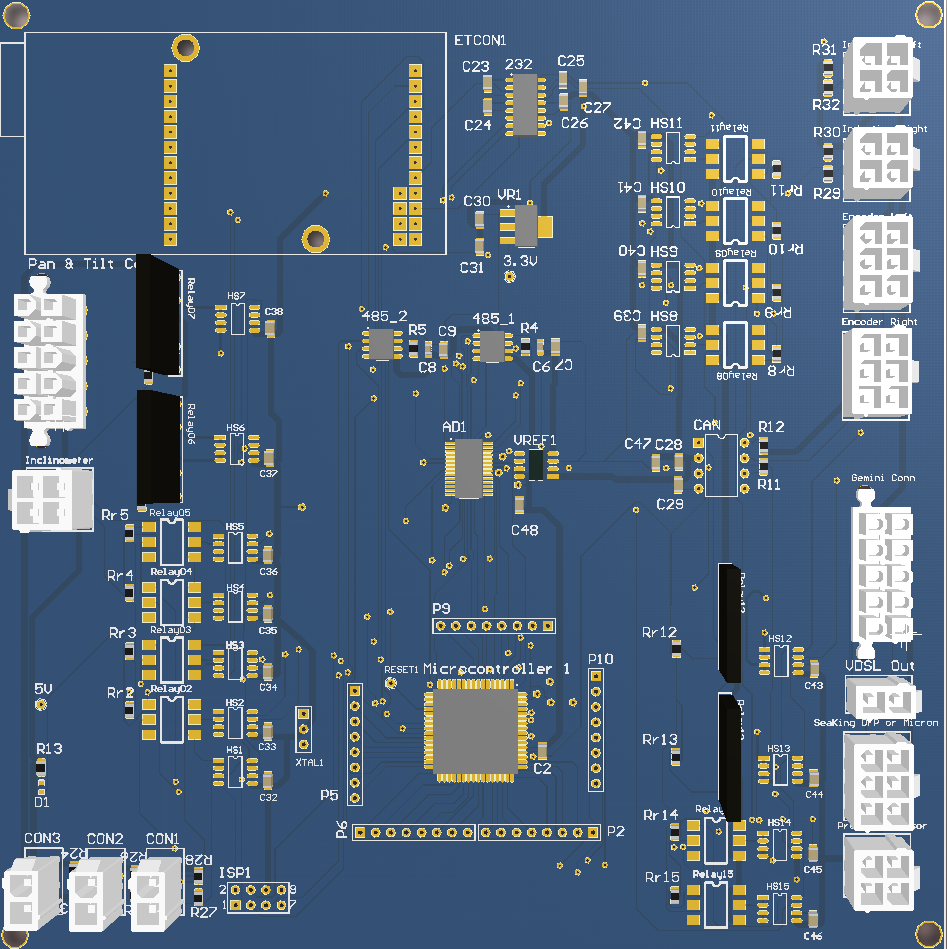
\includegraphics[width=0.5\columnwidth]{figs/eletronica/1.png}
    \caption{Placa 3D}
    \label{placa}
\end{figure}

\begin{figure}[H]
    \centering
    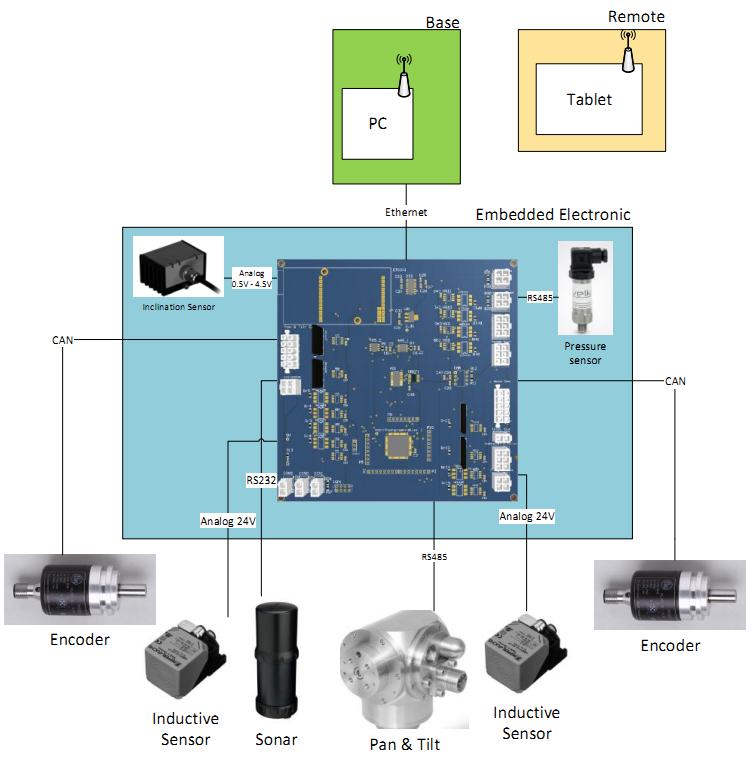
\includegraphics[width=0.5\columnwidth]{figs/eletronica/2.png}
    \caption{Diagrama de Alimentações}
    \label{alimentacao_placa}
\end{figure}

\begin{figure}[H]
    \centering
    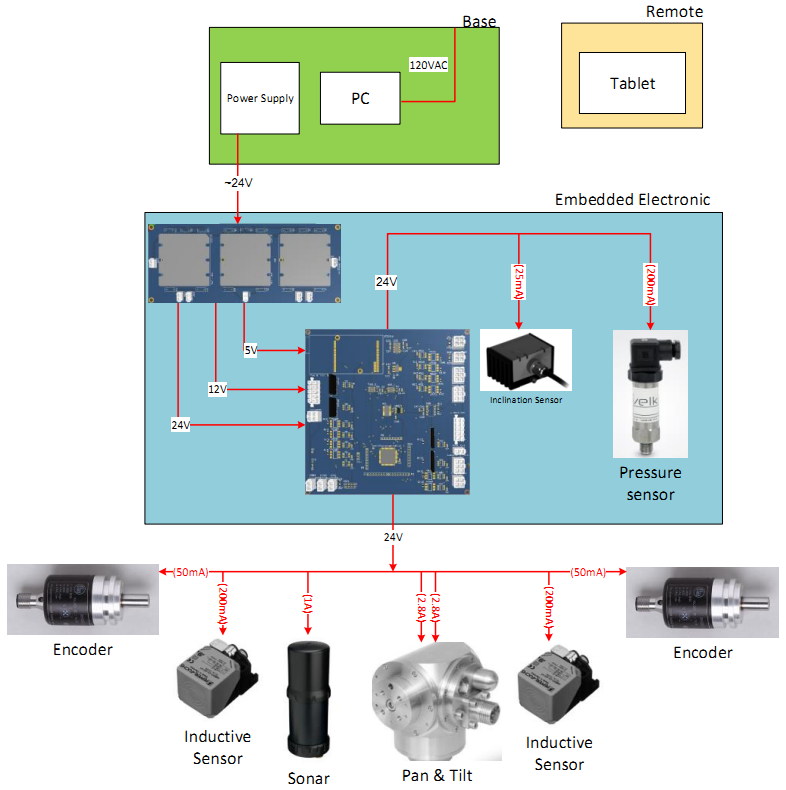
\includegraphics[width=0.5\columnwidth]{figs/eletronica/3.png}
    \caption{Diagrama de Comunicação}
    \label{com_placa}
\end{figure}
 
A placa com microcontrolador é uma solução de baixo custo, porém exige maior tempo de execução. Há a necessidade de fabricação, montagem, testes elétricos e lógicos da placa e programação de microcontrolador para gerenciamento de cada interface, como o protocolo CANOpen. 
A eletrônica deverá ser acoplada ao Lifting Beam, logo deverá ser construída uma estrutura mecânica à prova d’água para esta solução.

\subsection{Arquitetura de Software Proposta 1}
O sistema se divide em três grandes blocos que serão encapsulados separadamente
e se comunicarão entre si. A primeira parte consiste no sistema de eletrônica
embarcada composta pelos sensores e um equipamento de roteamento dos dados, a
segunda parte consiste no sistema de gerenciamento e processamento de dados em
terra e, finalmente, o último bloco consiste na camada de interface
homem-máquina , que consiste em um Tablet com sistema operacional Android.

Cada sensor deverá possuir um driver para a interface entre o equipamento físico
e camada de software, isto é, os encoders, inclinômetro, os sensores indutivos e
o sensor de pressão possuirão drivers dedicados para a leitura de dados, feita
através de uma conexão Ethernet para a placa que interconecta os sensores. O
sonar e o módulo PanTilt também possuirão drivers próprios para a aquisição de
dados e controle.

Nesta proposta, após a aquisição de dados, a placa embarcada realizará o
roteamento e envio de todos os dados para o computador em terra por meio do
driver do módulo Ethernet.  Os dados transmitidos pela eletrônica embarcada são
separados em dois grandes grupos: referentes à Monitoração e os referentes à
Visualização Sonar.

No computador localizado em terra, o componente de software responsável pela
monitoração irá processar e conformar os dados provenientes dos sensores
utilizados para o monitoramento das operações de inserção e remoção (encoders,
inclinômetro, sensores indutivos e sensor de pressão). Os dados provenientes do
sonar devem ser integrados com a posição do elemento PanTilt, no componente
Sonar-PanTilt, para que sejam consistentes e completos.  O módulo de
Reconstrução 3D é responsável, então, por traduzir os dados processados pelo
componente anterior em uma visualização inteligível para o ser humano.  Um
componente de segurança também é adicionado para monitorar a correta utilização
do sonar (apenas embaixo d’água), conferindo uma maior robustez ao sistema.

Ambos os componentes de processamento e conformação de dados, Monitoração e
Visualização Sonar, irão se comunicar com o Tablet com sistema operacional
Android por meio do componente Transmissão de dados – Tablet, enviando os dados
processados e recebendo os comandos de controle.  A interface homem máquina
consiste em um aplicativo cuja finalidade é realizar a interface do sistema com
o usuário, possibilitando uma correta e fácil visualização de todas as
informações pertinentes do sistema e suas operações.

\subsection{Arquitetura de Software Proposta 1}
O sistema se divide em três grandes blocos que serão encapsulados separadamente e se comunicarão entre si. A primeira parte consiste no sistema de eletrônica embarcada composta pelos sensores e um equipamento de roteamento dos dados, a segunda parte consiste no sistema de gerenciamento e processamento de dados em terra e, finalmente, o último bloco consiste na camada de interface homem-máquina , que consiste em um Tablet com sistema operacional Android.
Cada sensor deverá possuir um driver para a interface entre o equipamento físico e camada de software, isto é, os encoders, inclinômetro, os sensores indutivos e o sensor de pressão possuirão drivers dedicados para a leitura de dados, feita através de uma conexão Ethernet para a placa que interconecta os sensores. O sonar e o módulo PanTilt também possuirão drivers próprios para a aquisição de dados e controle. 
Nesta proposta, após a aquisição de dados, a placa embarcada realizará o roteamento e envio de todos os dados para o computador em terra por meio do driver do módulo Ethernet.  Os dados transmitidos pela eletrônica embarcada são separados em dois grandes grupos: referentes à Monitoração e os referentes à Visualização Sonar. 
No computador localizado em terra, o componente de software responsável pela monitoração irá processar e conformar os dados provenientes dos sensores utilizados para o monitoramento das operações de inserção e remoção (encoders, inclinômetro, sensores indutivos e sensor de pressão). Os dados provenientes do sonar devem ser integrados com a posição do elemento PanTilt, no componente Sonar-PanTilt, para que sejam consistentes e completos.  O módulo de Reconstrução 3D é responsável, então, por traduzir os dados processados pelo componente anterior em uma visualização inteligível para o ser humano.  Um componente de segurança também é adicionado para monitorar a correta utilização do sonar (apenas embaixo d’água), conferindo uma maior robustez ao sistema. 
Ambos os componentes de processamento e conformação de dados, Monitoração e Visualização Sonar, irão se comunicar com o Tablet com sistema operacional Android por meio do componente Transmissão de dados – Tablet, enviando os dados processados e recebendo os comandos de controle.  A interface homem máquina consiste em um aplicativo cuja finalidade é realizar a interface do sistema com o usuário, possibilitando uma correta e fácil visualização de todas as informações pertinentes do sistema e suas operações.


\section{Proposta 2 – PC Embarcado e base com Roteador}

A solução com um PC embarcado, acoplado à estrutura do Lifting Beam, é
considerada uma solução intermediária em relação ao custo e é uma solução que
mais se aproxima ao produto final. Esta solução é menos suscetível a falhas
elétricas e de gerenciamento de dispositivos, quando comparada com a solução da
placa com microcontrolador. Além disso, o tempo de execução gasto para programação de microcontrolador e fabricação da placa justifica a aquisição de um PC104. Na figura~\ref{pc104}, podemos observar o diagrama de interfaces desta solução.

\begin{figure}[H]
    \centering
    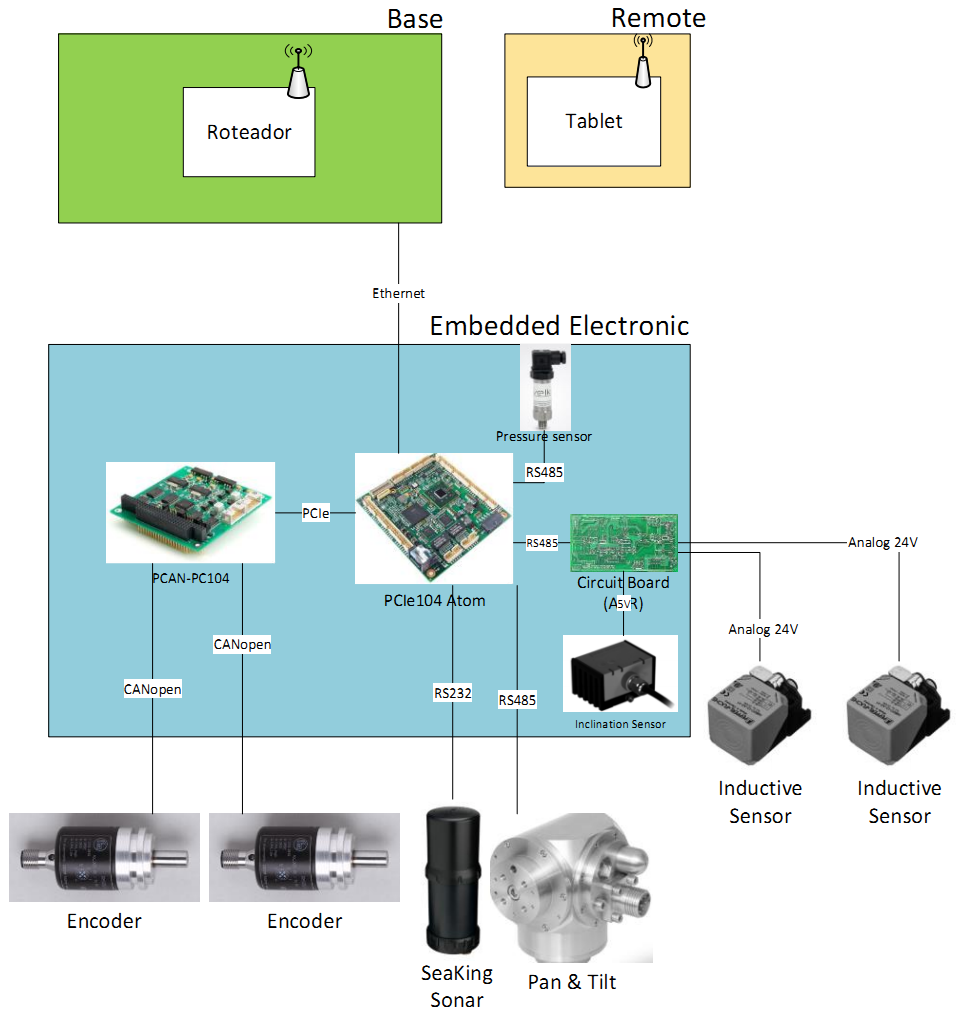
\includegraphics[width=0.5\columnwidth]{figs/eletronica/4.png}
    \caption{Diagrama de Comunicações - PC104}
    \label{pc104}
\end{figure} 
 
Assim como a solução 1, deverá ser construída uma estrutura mecânica à prova d’água.

subsection{Arquitetura de Software Proposta 2}

Para esta proposta o processamento dos dados aquisitados pelos sensores será
processado na própria eletrônica embarcada e, em seguida,
 serão enviados para o tablet, podendo ser roteado por um computador em terra ou
 diretamente por um roteador.
 
Cada sensor deverá possuir, novamente, um driver para a interface entre o
equipamento físico e camada de software,
 isto é, os encoders, inclinômetro, os sensores indutivos e o sensor de pressão
 possuirão drivers dedicados para a leitura de dados,
feita através de uma conexão Ethernet para a placa que interconecta os sensores.
O sonar e o módulo PanTilt também possuirão drivers próprios para a aquisição de
dados e controle.

Todos os componentes principais estão localizados no computador embarcado.
O componente de software responsável pela monitoração irá processar e conformar
os dados provenientes dos sensores utilizados para o monitoramento das operações
de inserção e remoção (encoders, inclinômetro, sensores indutivos
 e sensor de pressão). Os dados provenientes do sonar devem ser integrados com a
 posição do elemento PanTilt,
  no componente Sonar-PanTilt, para que sejam consistentes e completos.  O
  módulo de Reconstrução 3D é responsável,
   então, por traduzir os dados processados pelo componente anterior em uma
   visualização inteligível para o ser humano.
Um componente de segurança também é adicionado para monitorar a correta
utilização do sonar (apenas embaixo d’água), conferindo uma maior robustez ao
sistema.

Após o processamento dos dados, será estabelecida uma conexão wi-fi com o tablet
por meio de um computador em terra ou
 apenas por meio de um roteador.
 
Os componentes da interface homem máquina permanecem inalterados em relação à
proposta anterior.


\subsection{Arquitetura de Software Proposta 2}

Para esta proposta o processamento dos dados aquisitados pelos sensores será
processado na própria eletrônica embarcada e, em seguida,
 serão enviados para o tablet, podendo ser roteado por um computador em terra ou
 diretamente por um roteador.
 
Cada sensor deverá possuir, novamente, um driver para a interface entre o
equipamento físico e camada de software,
 isto é, os encoders, inclinômetro, os sensores indutivos e o sensor de pressão
 possuirão drivers dedicados para a leitura de dados,
feita através de uma conexão Ethernet para a placa que interconecta os sensores.
O sonar e o módulo PanTilt também possuirão drivers próprios para a aquisição de
dados e controle.

Todos os componentes principais estão localizados no computador embarcado.
O componente de software responsável pela monitoração irá processar e conformar
os dados provenientes dos sensores utilizados para o monitoramento das operações
de inserção e remoção (encoders, inclinômetro, sensores indutivos
 e sensor de pressão). Os dados provenientes do sonar devem ser integrados com a
 posição do elemento PanTilt,
  no componente Sonar-PanTilt, para que sejam consistentes e completos.  O
  módulo de Reconstrução 3D é responsável,
   então, por traduzir os dados processados pelo componente anterior em uma
   visualização inteligível para o ser humano.
Um componente de segurança também é adicionado para monitorar a correta
utilização do sonar (apenas embaixo d’água), conferindo uma maior robustez ao
sistema.

Após o processamento dos dados, será estabelecida uma conexão wi-fi com o tablet
por meio de um computador em terra ou
 apenas por meio de um roteador.
 
Os componentes da interface homem máquina permanecem inalterados em relação à
proposta anterior.
 

\section{Proposta 3 – PC embarcado e PC na base}

A terceira solução consiste na compra de uma eletrônica embarcada e um
computador em Pelican Case. Esta solução, apesar de ser a mais custosa, é mais
robusta devido ao grau de proteção elétrica e mecânica, além de já estar em
conformidade quanto aos requisitos de projeto.

\subsubsection{Arquitetura de Software Proposta 3}
Esta proposta é um meio termo entre a proposta com todo o processamento em terra
(proposta 1) e a proposta anterior, na qual todo o processamento de dados se dá
na eletrônica embarcada. Os componentes de software são basicamente os mesmos,
excetuando-se a ordem em que o processamento e a comunicação ocorrem.

Os dados dos sensores das operações de inserção e remoção de Stoplogs
(encoders, inclinômetro, sensores indutivos e sensor de pressão), assim como os
dados brutos provenientes do sonar e do módulo PanTilt serão conformados em um
computador embarcado e enviados via ethernet para um computador em superfície.

Já na superfície o componente Sonar-PanTilt realizará a fusão dos dados
referentes ao sonar e o módulo de reconstrução 3D irá gerar a imagem,
analogamente as outras propostas. Por fim os componentes de Monitoração e
Visualização enviarão os dados processados para o tablet. O componente de
segurança também está implementado no computador em terra.

A maior vantagem dessa arquitetura, na ótica de software, é a facilidade de
manutenção, uma vez que para a realização de qualquer alteração do software do
sistema não é necessário a abertura da envólucro do sistema embarcado. Já a sua
desvantagem seria a maior quantidade de trabalho para a programação de dois
sistemas.

\section{Estágio atual do projeto}

Concluído:
\begin{itemize}
  \item Projeto conceitual;
  \item Pesquisa, compra e recebimento de sensores Indutivos;
  \item Pesquisa, compra e recebimento de encoders;
  \item Pesquisa e compra de Sonar (importação);
  \item Pesquisa e compra de sistema Pan & Tilt (importação);
  \item Pesquisa e compra de sensor de Pressão;
  \item Teste com sensores indutivos;
  \item Pesquisa, compra e recebimento de Tablet;
  \item Projetos de placas com microcontrolador;
  \item Projeto de placa com conversores para alimentação elétrica;
  \item Pesquisa de PC104 e acessórios;   
\end{itemize}
Em andamento:
\begin{itemize}
  \item Aplicativo para interface do sistema com usuário.
  \item Compra de PC104 e acessórios para a solução 2.
  \item Revisão da placa.
  \item Set-up para teste de bancada com sonar.
\end{itemize}